\documentclass{beamer}
\mode<presentation>
\usepackage{amsmath}
\usepackage{amssymb}
%\usepackage{advdate}
\usepackage{adjustbox}
\usepackage{subcaption}
\usepackage{enumitem}
\usepackage{multicol}
\usepackage{mathtools}
\usepackage{listings}
\usepackage{url}
\def\UrlBreaks{\do\/\do-}
\usetheme{metropolis}
\setbeamertemplate{footline}
{
  \leavevmode%
  \hbox{%
  \begin{beamercolorbox}[wd=\paperwidth,ht=2.25ex,dp=1ex,right]{author in head/foot}%
    \insertframenumber{} / \inserttotalframenumber\hspace*{2ex} 
  \end{beamercolorbox}}%
  \vskip0pt%
}
\setbeamertemplate{navigation symbols}{}

\providecommand{\nCr}[2]{\,^{#1}C_{#2}} % nCr
\providecommand{\nPr}[2]{\,^{#1}P_{#2}} % nPr
\providecommand{\mbf}{\mathbf}
\providecommand{\pr}[1]{\ensuremath{\Pr\left(#1\right)}}
\providecommand{\qfunc}[1]{\ensuremath{Q\left(#1\right)}}
\providecommand{\sbrak}[1]{\ensuremath{{}\left[#1\right]}}
\providecommand{\lsbrak}[1]{\ensuremath{{}\left[#1\right.}}
\providecommand{\rsbrak}[1]{\ensuremath{{}\left.#1\right]}}
\providecommand{\brak}[1]{\ensuremath{\left(#1\right)}}
\providecommand{\lbrak}[1]{\ensuremath{\left(#1\right.}}
\providecommand{\rbrak}[1]{\ensuremath{\left.#1\right)}}
\providecommand{\cbrak}[1]{\ensuremath{\left\{#1\right\}}}
\providecommand{\lcbrak}[1]{\ensuremath{\left\{#1\right.}}
\providecommand{\rcbrak}[1]{\ensuremath{\left.#1\right\}}}
\theoremstyle{remark}
\newtheorem{rem}{Remark}
\newcommand{\sgn}{\mathop{\mathrm{sgn}}}
\providecommand{\abs}[1]{\left\vert#1\right\vert}
\providecommand{\res}[1]{\Res\displaylimits_{#1}} 
\providecommand{\norm}[1]{\lVert#1\rVert}
\providecommand{\mtx}[1]{\mathbf{#1}}
\providecommand{\mean}[1]{E\left[ #1 \right]}
\providecommand{\fourier}{\overset{\mathcal{F}}{ \rightleftharpoons}}
%\providecommand{\hilbert}{\overset{\mathcal{H}}{ \rightleftharpoons}}
\providecommand{\system}{\overset{\mathcal{H}}{ \longleftrightarrow}}
	%\newcommand{\solution}[2]{\textbf{Solution:}{#1}}
%\newcommand{\solution}{\noindent \textbf{Solution: }}
\providecommand{\dec}[2]{\ensuremath{\overset{#1}{\underset{#2}{\gtrless}}}}
\newcommand{\myvec}[1]{\ensuremath{\begin{pmatrix}#1\end{pmatrix}}}
\let\vec\mathbf

\lstset{
%language=C,
frame=single, 
breaklines=true,
columns=fullflexible
}

\numberwithin{equation}{section}

\title{Solution to DES using Laplace Transforms}
\author{Aditya Tripathy\\ Dept. of Electrical Engg.,\\IIT Hyderabad.}

\date{\today} 
\begin{document}

\begin{frame}
\titlepage
\end{frame}

\section*{Outline}
\begin{frame}
\frametitle{Table Of Contents}
\tableofcontents
\end{frame}
\section{Problem}
\begin{frame}
\frametitle{Problem Statement}
%

Plot the solution to $y^\prime + 2y = \sin x$
%A circle $C$ passes through 
%\begin{equation} 
%\vec{P}=\myvec{-2\\ 4} 
%\label{eq:circle_7_p}
%\end{equation} 
%and touches the $y$-axis at 
%\begin{equation} 
%\vec{Q}=\myvec{0\\ 2}. 
%\label{eq:circle_7_q}
%\end{equation}
%Which one of the  following equations can represent a diameter of this circle?
%\begin{enumerate}[label=(\roman*)]
%\begin{multicols}{2}
%\setlength\itemsep{1em}
%\item $\myvec{4 & 5}\vec{x} = 6 $
%\item $\myvec{2 & -3}\vec{x} +10 = 0 $
%\item $\myvec{3 & 4}\vec{x} = 3 $
%\item $\myvec{5 & 2}\vec{x} +4= 0 $
%\end{multicols}
%\end{enumerate}
\end{frame}

%\subsection{Literature}
\section{Solution}
\subsection{Discretizing}
\begin{frame}
\frametitle{Euler's Method}
To plot a curve in the solution family, we take the initial condition to be\\
$x_0 = 0, y_0 = 1$\\
Using Euler's Method, we represent the the differential equation in the following difference equations:
\begin{align}
    x_{n+1} = x_n + h\\
    y_{n+1} - y_n + 2hy_n  = h\sin x_n\\
    \xrightarrow{} y_{n+1} = \brak{1-2h}y_n + h\sin x_n
\end{align}
Now we can iteratively generate points which lie close to the graph.\\

%\framesubtitle{Literature}
%Let $\vec{O}$ be the centre of $C$. Then the equation of the normal, OQ is
%\begin{align}
%%\vec{x}^T\vec{x}-2\vec{O}^T\vec{x} +F = 0
%\myvec{0 & 1}\brak{\vec{O}-\vec{Q}} &= 0
%\nonumber \\ 
%\implies \myvec{0 & 1}\vec{O} = 2
%\label{eq:circle_7_o1}
%\end{align}
%%
%Also, 
%%Substituting \eqref{eq:circle_7_p} in \eqref{eq:circle_7_c}, 
%\begin{align}
%\norm{\vec{O}-\vec{P}}^2&=\norm{\vec{O}-\vec{Q}}^2 
%\nonumber \\
%\implies 2\brak{\vec{P}-\vec{Q}}^T\vec{O} &= \norm{\vec{P}}^2-\norm{\vec{Q}}^2 
%\nonumber \\
%\text{or, } \myvec{1 & -1}\vec{O} &= -4
%\label{eq:circle_7_o2}
%\end{align}
%%
%\eqref{eq:circle_7_o1} and \eqref{eq:circle_7_o2} result in the matrix equation
%\begin{align}
%\myvec{1 & -1 \\ 0 & 1}\vec{O} = \myvec{-4\\2}
%\label{eq:circle_7_matrix}
%\end{align}
%yielding the augmented matrix
%\begin{align}
%\myvec{1 & -1 & -4\\ 0 & 1 & 2} \leftrightarrow \myvec{1 & 0 & -2\\ 0 & 1 & 2}\implies \vec{O} = \myvec{-2 \\2}
%\label{eq:circle_7_o}
%\end{align}
%%
\end{frame}
\subsection{Theoretical Solution}
\begin{frame}
\frametitle{Laplace Transform}
Let $\mathcal{L}\brak{y} = Y$\\
\begin{align}
    \brak{sY - y_0} +2Y &= \mathcal{L}\brak{\sin x}\\
    \mathcal{L}\brak{\sin x} &= \int_{0}^{\infty} e^{-sx}\sin x = \frac{1}{s^2 + 1}\\
    \brak{s + 2}Y &= y_0 + \frac{1}{s^2 + 1}\\
    Y &= \frac{y_0}{s + 2} + \frac{1}{\brak{s^2+1}\brak{s+2}}\\
\end{align}
%\begin{enumerate}[label=(\roman*)]
%\item $\myvec{4 & 5}\vec{O} = 2 \ne 6 $. Incorrect.
%\vfill
%\item $\myvec{2 & -3}\vec{O} +10 = 0 $. Correct.
%\vfill
%\item $\myvec{3 & 4}\vec{O} = 2 \ne 3 $.  Incorrect.
%\vfill
%\item $\myvec{5 & 2}\vec{O} +4= -2 \ne 0 $. Incorrect
%\end{enumerate}

\end{frame}
\begin{frame}
\frametitle{Laplace Transform}
 Using method of partial fractions,
    \begin{align}   
        \frac{1}{\brak{s^2+1}{s+2}} = \frac{a}{s+2} + \frac{bs + c}{s^2+1}\\
    \end{align}
    On solving we get,
    \begin{align}
        a &= \frac{1}{5}\\
        b &= \frac{-1}{5}\\
        c &= \frac{2}{5}\\
    \end{align}
    \text{Substituting $y_0 = 1$},\\
\end{frame}
\begin{frame}
\frametitle{Laplace Transform}
\begin{align}
    Y &= \frac{1}{s + 2} + \frac{0.2}{s+2} + \frac{-0.2s}{s^2 + 1} + \frac{0.4}{s^2 + 1}\\
    \xrightarrow{} Y &=  \frac{1.2}{s + 2} + \frac{-0.2s}{s^2 + 1} + \frac{0.4}{s^2 + 1}\\
\end{align}
    \text{Now, we take the inverse laplace transform to get a solution,}\\
\begin{align}
    \mathcal{L}^{-1}\brak{\frac{1}{s+2}} &= e^{-2x}u\brak{x}\\
    \mathcal{L}^{-1}\brak{\frac{1}{s^2+1}} &= \sin xu\brak{x}\\
    \mathcal{L}^{-1}\brak{\frac{s}{s^2+1}} &= \cos xu\brak{x}
\end{align}

\end{frame}
\begin{frame}
\frametitle{Laplace Transform}
Therefore the final solution to the differential equation is,
\begin{align}
    y\brak{x} = \brak{1.2e^{-2x} - 0.2\cos x + 0.4\sin x}u\brak{x}
\end{align}
\end{frame}

%\section{Plot}
\subsection{Graph}
\begin{frame}[fragile]
\frametitle{Graph}
\begin{figure}[h!]
   \centering
   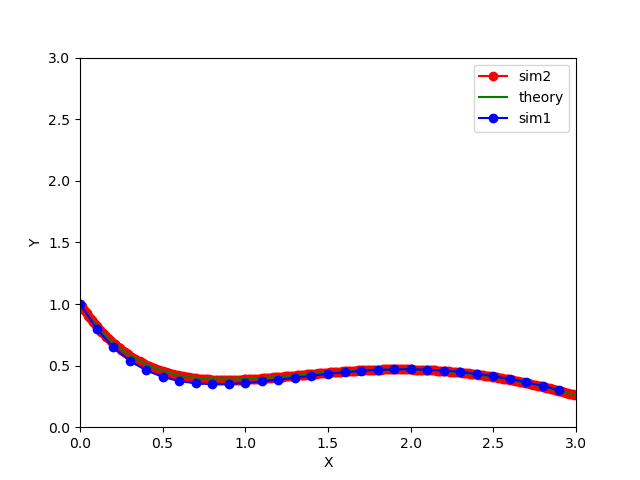
\includegraphics[width=0.7\linewidth]{figs/fig.png}
   \caption{equilateral triangle of side 5cm}
\end{figure}
\end{frame}
\end{document}
